\documentclass[degree=master,fontset=windows]{thuthesis}
% \documentclass[fontset=mac]{thuthesis}
  % 学位 degree:
  %   doctor | master | bachelor | postdoc
  % 学位类型 degree-type:
  %   academic（默认）| professional
  % 语言 language
  %   chinese（默认）| english
  % 字体库 fontset
  %   windows | mac | fandol | ubuntu
  % 建议终版使用 Windows 平台的字体编译
% 论文基本配置，加载宏包等全局配置


\newcommand{\midsepremove}{\aboverulesep=0pt \belowrulesep=0pt}
\usepackage{xcolor}
\newcommand{\graycell}[1]{
  \setlength{\fboxsep}{0.5pt}
  \colorbox{gray!20}{\makebox[2.75em][c]{#1}}
}

\input{thusetup}
\usepackage{setspace}
\begin{document}
% 封面
% 学位论文封面页
\begin{titlepage}

\noindent\textbf{\zihao{4}{分类号：{\normalfont TP183}} \hspace*{180pt} {学校代码：{\normalfont 10423}} \\ 
{UDC：{\normalfont 004.8}} \hspace*{206pt} {学~~~~~号：{\normalfont 21220213161}}}
\vskip50pt
\par \vskip20pt

% 中文标题
\begin{spacing}{1.5}
\centering{\fontsize{22pt}{30pt}\selectfont\heiti 面向人脸视频伪造检测的时空建模方法}
\par \vskip30pt
\ctitle{面向人脸视频伪造检测的时空建模方法}
% 英文标题
\centering{\fontsize{22pt}{80pt}\selectfont\textbf{Face Forgery Video Detection via Spatio-Temporal Modeling}}
\end{spacing}

% 作者
\par\vskip110pt
{~~~~~~~~~~~~~~~~~~~~~~ \ziju{0.65}\fontsize{14pt}{21pt}\selectfont\heiti 作 ~~~~~~~~~~~~~~ 者：}
{\fontsize{14pt}{21pt}\selectfont 刘英杰}

% 指导教师
\par\vskip6pt
{~~~~~~~~~~~~~~~~~~~~~~ \ziju{0.65}\fontsize{14pt}{21pt}\selectfont\heiti 指导教师：}
{\fontsize{14pt}{21pt}\selectfont 郑海永 、郭宗辉}
% 合作导师
\par\vskip6pt
% {~~~~~~~~~~~~~~~~~~~~~~ \ziju{0.65}\fontsize{14pt}{21pt}\selectfont\heiti 合作导师：}
% {\fontsize{14pt}{21pt}\selectfont 郭宗辉 ~ 副教授}
% % 学位类型
% \par\vskip6pt
{~~~~~~~~~~~~~~~~~~~~~~ \ziju{0.65}\fontsize{14pt}{21pt}\selectfont\heiti 学位类型：}
{\fontsize{14pt}{21pt}\selectfont 专业学位}

% 专业名称
\par\vskip6pt
{~~~~~~~~~~~~~~~~~~~~~~ \ziju{0.65}\fontsize{14pt}{21pt}\selectfont\heiti 专业名称：}
{\fontsize{14pt}{21pt}\selectfont 新一代电子信息技术}

% 研究方向
\par\vskip6pt
{~~~~~~~~~~~~~~~~~~~~~~ \ziju{0.65}\fontsize{14pt}{21pt}\selectfont\heiti 研究方向：}
{\fontsize{14pt}{21pt}\selectfont 信号与信息智能处理}

% 
\par\vskip6pt
{~~~~~~~~~~~~~~~~~~~~~~ \fontsize{14pt}{21pt}\selectfont\heiti 授予学位单位：}{\fontsize{14pt}{21pt}\selectfont ~中国海洋大学}

\par\vskip80pt
\centering{\fontsize{14}{32}\selectfont\heiti 日期：~~~ 2025 ~~~ 年 ~~~5 ~~~ 月 ~~~ 13 ~~~日 }

\end{titlepage}

\include{data/committee.tex}
% 学位论文独创声明
% 学位论文独创声明
\begin{titlepage}
\newgeometry{left=2.5cm, right=2.5cm, top=2.5cm, bottom=2.5cm} % 调整当前页的页边距
\newpage % 切换到新页以应用新的页边距

\par\vskip30pt
\begin{spacing}{1.5}
\centering{\fontsize{16pt}{24pt}\selectfont\heiti 学位论文独创声明}
\end{spacing}



\par\vskip20pt
\begin{spacing}{1.25}
本人所呈交的学位论文是本人在导师指导下进行的研究工作及取得的研究成果。除了文中加以标注和致谢的地方外，论文中不包含其他人已经发表或撰写过的研究成果，也不包含为获得\underline{~~~~~~~~~~~~~~~~~~~~~~~（注：如没有其他需要特别声明的，本栏可空）}或其他教育机构的学位或证书使用过的材料。对本文的研究作出重要贡献的个人和集体，均已在文中以明确方式标明。本声明的法律责任由本人承担。
\end{spacing}
\par\vskip60pt

学位论文作者签名：\hspace*{160pt} 日期：

\begin{spacing}{1.5}
\centering{- - - - - - - - - - - - - - - - - - - - - - - - - - - - - - - - - - - - - - - - - - - - - - - - - - - - - - - - - }
\end{spacing}

\begin{spacing}{1.5}
\centering{\fontsize{16pt}{24pt}\selectfont\heiti 学位论文版权使用授权书}
\end{spacing}

\par\vskip20pt
\begin{spacing}{1.25}
本学位论文作者完全了解国家有关保留、使用学位论文的法律、法规和学校有关规定，并同意以下事项：

1.学校有权保留并向国家有关部门或机构送交本学位论文的复印件和电子版，允许论文被查阅和借阅；

2.学校可以将本学位论文的全部或部分内容编入有关数据库进行检索，可以采用影印、缩印或扫描等复制手段保存、汇编本学位论文；

3.学校可以基于教学及科研需要合理使用本学位论文。

需保密的学位论文在解密后适用本授权书。
\end{spacing}
\par\vskip60pt
学位论文作者签名：\hspace*{160pt} 导师签名：
\par\vskip20pt
日期： \hspace*{231pt} 日期：
\restoregeometry % 恢复原来的页边距
\newpage % 切换到新页以恢复原来的页边距
\end{titlepage}



% \begin{titlepage}

% \par\vskip30pt
% \begin{spacing}{1.5}
% \centering{\fontsize{16pt}{24pt}\selectfont\heiti 学位论文独创声明}
% \end{spacing}

% \par\vskip20pt
% 本人所呈交的学位论文是本人在导师指导下进行的研究工作及取得的研究成果。除了文中加以标注和致谢的地方外，论文中不包含其他人已经发表或撰写过的研究成果，也不包含为获得\underline{~~~~~~~~~~~~~~~~~~~~~~~（注：如没有其他需要特别声明的，本栏可空）}或其他教育机构的学位或证书使用过的材料。对本文的研究作出重要贡献的个人和集体，均已在文中以明确方式标明。本声明的法律责任由本人承担。

% \par\vskip60pt

% 学位论文作者签名：\hspace*{160pt} 日期：

% \begin{spacing}{1.5}
% \centering{- - - - - - - - - - - - - - - - - - - - - - - - - - - - - - - - - - - - - - - - - - - - - - - - - - - - - - - - - }
% \end{spacing}

% \begin{spacing}{1.5}
% \centering{\fontsize{16pt}{24pt}\selectfont\heiti 学位论文版权使用授权书}
% \end{spacing}

% \par\vskip20pt
% 本学位论文作者完全了解国家有关保留、使用学位论文的法律、法规和学校有关规定，并同意以下事项：

% 1.学校有权保留并向国家有关部门或机构送交本学位论文的复印件和电子版，允许论文被查阅和借阅；

% 2.学校可以将本学位论文的全部或部分内容编入有关数据库进行检索，可以采用影印、缩印或扫描等复制手段保存、汇编本学位论文；

% 3.学校可以基于教学及科研需要合理使用本学位论文。

% 需保密的学位论文在解密后适用本授权书。

% \par\vskip60pt
% 学位论文作者签名：\hspace*{160pt} 导师签名：
% \par\vskip20pt
% 日期： \hspace*{231pt} 日期：

% \end{titlepage}

% 英文目录映射
\makeatletter
\newcommand\engcontentsname{Contents}
\newcommand\tableofengcontents{%
  \pagestyle{plain}
  % \pagenumberingnoreset{Roman}
    \fancyhf{} % 清除所有默认页眉页脚
    \fancyfoot[C]{\thepage} % 页码居中
    \renewcommand{\headrulewidth}{0pt} % 去掉页眉横线
  \setcounter{tocdepth}{3} 
  \chapter*{\bfseries \engcontentsname}%
  \@starttoc{toe}%
  \clearpage
}
\newcommand\addengcontents[2]{%
    \addcontentsline{toe}{#1}{\protect\numberline{\csname the#1\endcsname}#2}}
\makeatother
\newcommand\addengcontent[2]{\addcontentsline{toe}{#1}{#2}}
% \newcommand\echapter[1]{\addengcontents{chapter}{#1}}
\newcommand\echapter[1]{
\addcontentsline{toe}{chapter}{\protect\numberline{\thechapter .}#1}}


\newcommand\esection[1]{\addengcontents{section}{#1}}
\newcommand\esubsection[1]{\addengcontents{subsection}{#1}}
\newcommand\esubsubsection[1]{\addengcontents{subsubsection}{#1}}
\newcommand\addengcontentsnonumber[2]{%
\addcontentsline{toe}{#1}{#2}}
% 使用授权的说明
% 本科生开题报告不需要

% \copyrightpage
% 将签字扫描后授权文件 scan-copyright.pdf 替换原始页面
% \copyrightpage[file=scan-copyright.pdf]
\frontmatter
\pagestyle{empty} % 取消所有页眉页脚（包括页码）


% !TeX root = ../thuthesis-example.tex

% 中英文摘要和关键字



\addengcontentsnonumber{chapter}{Abstract (In Chinese)}
\begin{abstract}
    摘要内容\\
  \noindent\textbf{关键词：}Transformer；
\end{abstract}


\begin{abstract*}
\addengcontentsnonumber{chapter}{Abstract (In English)}
    Abstract \\
  \noindent\textbf{Key Words：}Transformer;
\end{abstract*}


\pagestyle{empty}
% % 中文摘要
% \include{data/abstract_ch.tex}
% % 英文摘要
% \include{data/abstract_en.tex}


% 目录
\renewcommand{\headrulewidth}{0pt}
% \setlength{\headheight}{15pt}
% \setlength{\headsep}{5mm}



\tableofcontents
\tableofengcontents % 英文目录


\addengcontentsnonumber{chapter}{Figure list \& Table list}


\renewcommand{\headrulewidth}{0pt}
% 插图和附表清单
% \listoffigures           % 插图清单
% \listoftables            % 附表清单


\listoffiguresandtables  % 插图和附表清单
\chapter*{注释表} % 星号表示不编号

\addcontentsline{toc}{chapter}{注释表} % 添加到目录
\addengcontentsnonumber{chapter}{Abbreviation}
\begin{center}
\begin{tabular}{ccc} % 三列左对齐，第一列加粗
\toprule % 上横线
\textbf{英文缩写} & \textbf{英文全称} & \textbf{中文全称} \\
\midrule % 中间线
FFD & Face Forgery Detection & 人脸伪造检测 \\
\bottomrule % 下横线
\end{tabular}
\end{center}


\pagestyle{plain}
% 符号对照表
% \input{data/denotation}

% 重新设置页眉和
% \pagestyle{fancy} 
\renewcommand{\headrulewidth}{0.75pt}
% 正文部分
\mainmatter
% \newgeometry{left=2.5cm, right=2.5cm, top=2.5cm, bottom=2.5cm}

% \geometry{
%     paper=a4paper,
%     top=1.5cm,           % 上边距（包含页眉）
%     bottom=1.5cm,        % 下边距（包含页脚）
%     headheight=15pt,   % 页眉高度
%     headsep=15mm,      % 页眉到正文的距离
%     footskip=15mm,     % 页脚到正文的距离
% }
% \newgeometry{top=2cm}

\chapter{绪论}
\echapter{Introduction}
\label{cha:chapter1}
本章对全文的工作进行简要的概述，首先阐述研究课题的背景和实际应用中的重要性。随后对国内外相关研究的进展和不足进行了探讨。基于上述背景与现状，明确核心目标，并对研究内容和创新点进行阐述。最后，介绍论文的整体结构和各个章节的核心内容。
\section{研究背景及意义}
\esection{Background}
\section{国内外研究现状}
\esection{Related work}
\subsection{人脸伪造检测}
\esubsection{Face forgery detection}
\section{研究内容}
\esection{Research content}
\begin{figure}[h]
\centering
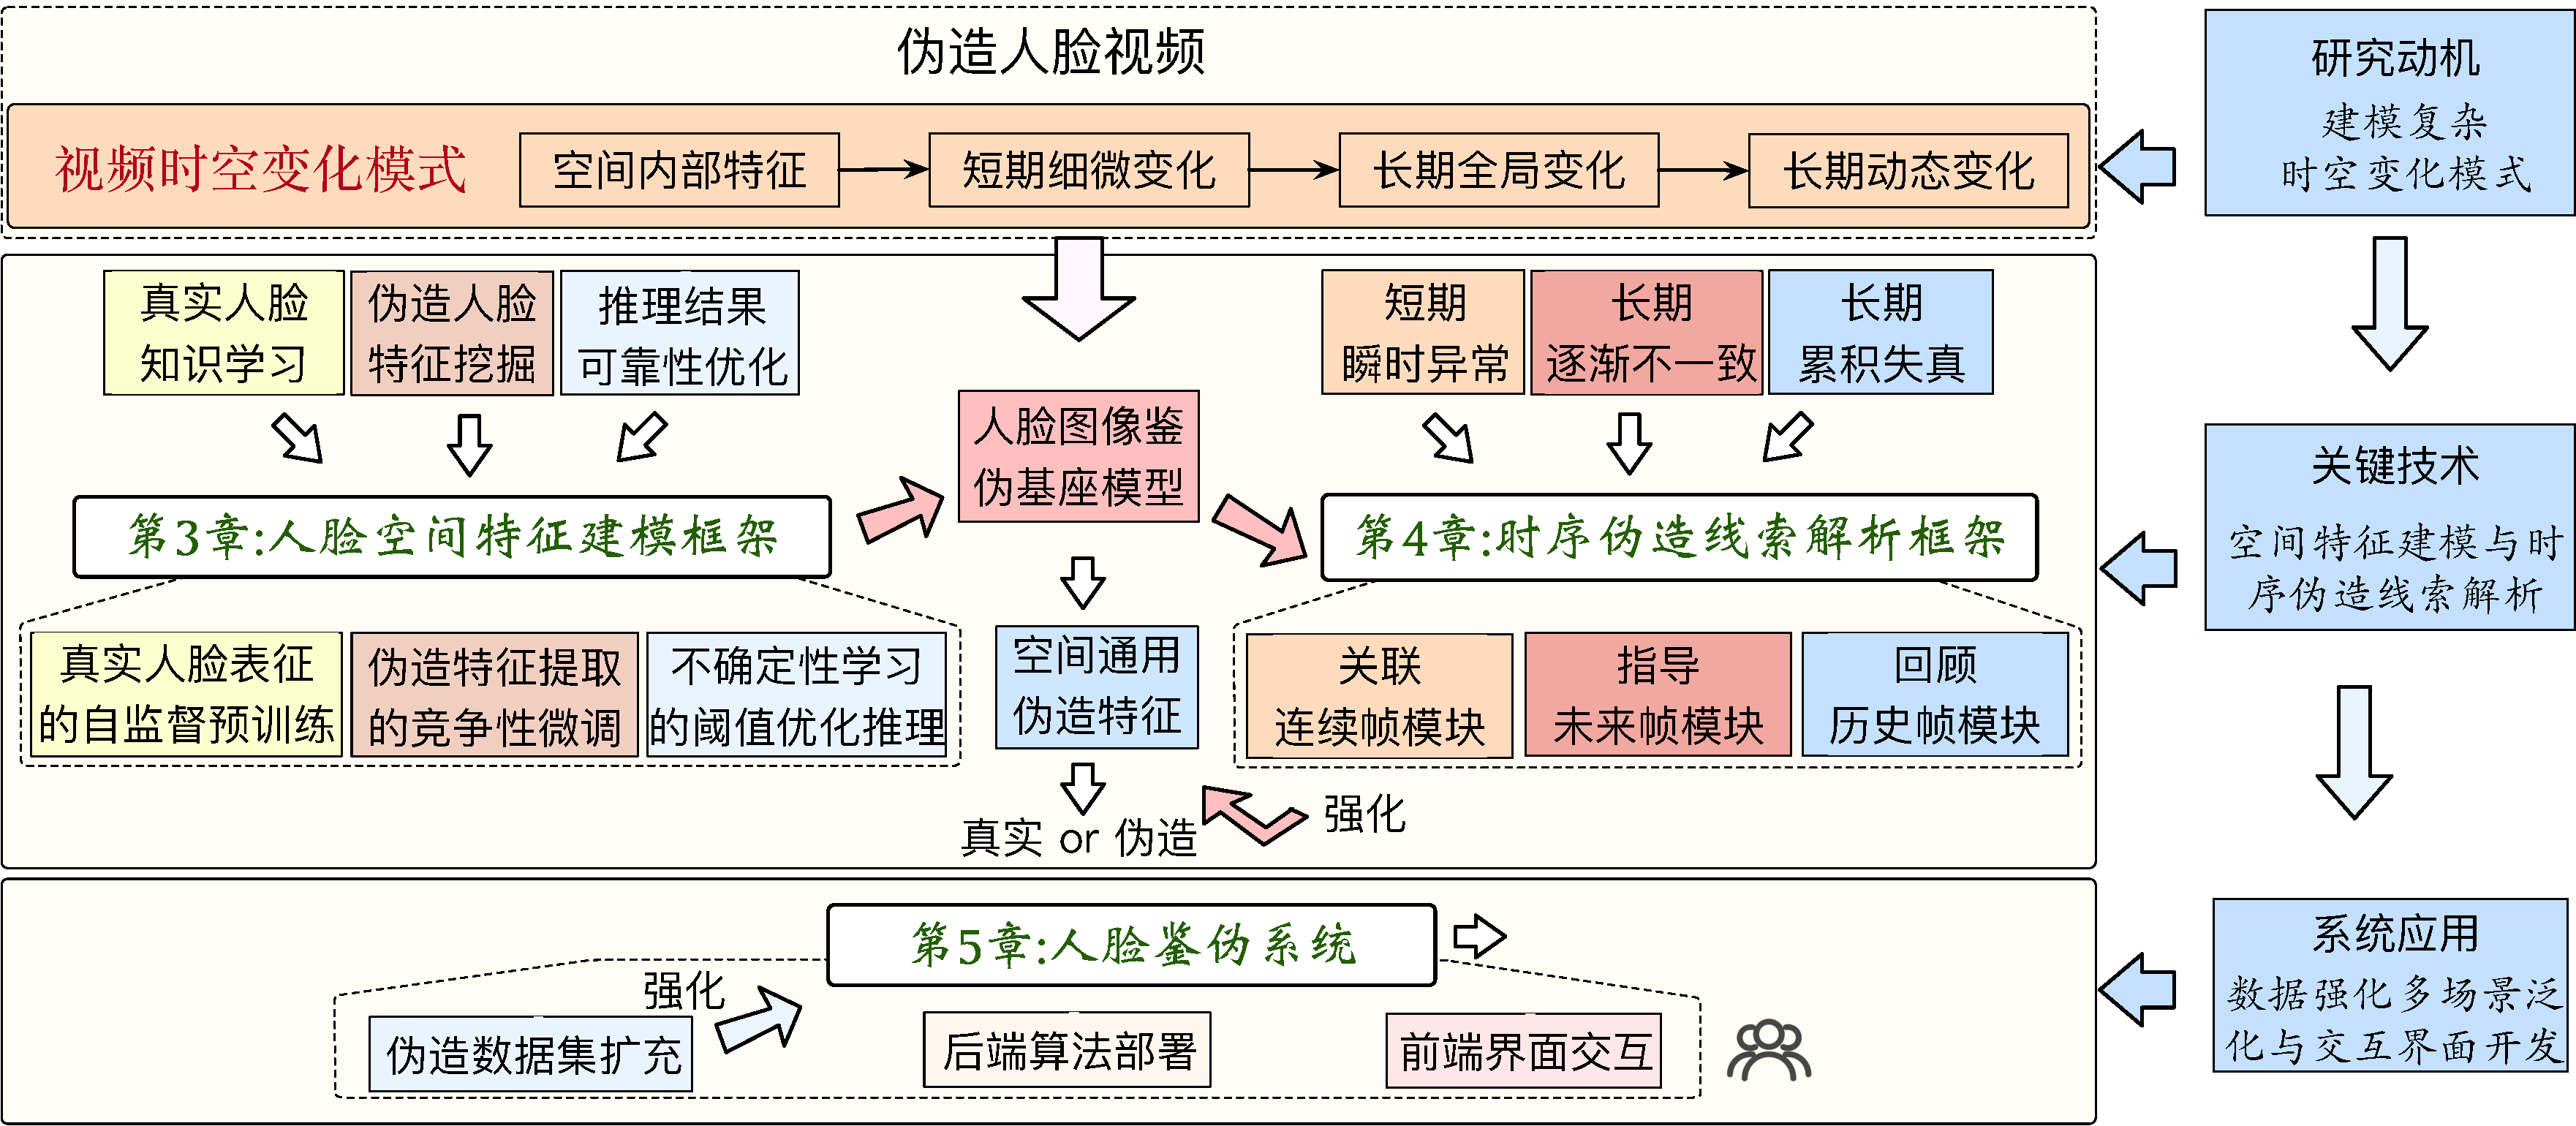
\includegraphics[width=1.0\linewidth]{fig/绪论.pdf}
\caption{本文的研究内容概览图}
\par\vspace{5pt}
\caption*{Figure \thefigure \ \ \ Overview of the research content of this thesis}
\label{fig:1-overview}
\end{figure}
\section{课题来源}
\esection{Research support}
国家自然科学基金面上项目“***”（批准号：***）。
\section{论文组织结构}
\esection{Paper structure}
本文聚焦于**，旨在**。组织结构如下：


第一章为绪论。首先介绍**任务的研究背景和意义；接着对国内外相关领域的研究现状和不足进行介绍；最后阐述本文的主要内容和贡献。




% \input{data/chap02}
% \input{data/chap03}
% \input{data/chap04}
% \include{data/chap05}
% \include{data/chap06}
% 参考文献
\bibliography{ref/refs}
% \bibliography{ref}  % 参考文献使用 BibTeX 编译
% \printbibliography       % 参考文献使用 BibLaTeX 编译

% 附录
% \appendix
% \input{data/appendix-survey}       % 本科生：外文资料的调研阅读报告
% \input{data/appendix-translation}  % 本科生：外文资料的书面翻译
% \input{data/appendix}

% 其他部分
\backmatter

% 致谢

% 声明
% 各类开题报告通常不需要
% \statement[page-style=empty]  % 编译生成的声明页默认不含页眉页脚，以避免页码变化带来问题
% 在提交终稿时，插入签字后的扫描件 scan-statement.pdf，并添加页眉页脚
% \statement[page-style=plain, file=scan-statement.pdf]
% 如确实需要在电子版中直接页眉页脚，则使用
% \statement[page-style=plain]

% 个人简历、在学期间完成的相关学术成果
% 本科生可以附个人简历，也可以不附个人简历
\begin{resume}

% \newcommand\addengcontentsnonumber[2]{%
%     \addcontentsline{toe}{#1}{#2}}
% \addengcontentsnonumber{chapter}{Published papers and research results while pursuing the degree}


%   \researchitem{发表的学术论文} % 发表的和录用的合在一起

%   % 1. 已经刊载的学术论文（本人是第一作者，或者导师为第一作者本人是第二作者）
%   \begin{publications}
%     \item [1]刘英杰，黄嘉琦，姜玉凤，邵宇琪，杨文韬，于紫凝，郑海永.融合电磁和地声特征的地震预测集成学习方法[J].计算机技术与发展,2024,34(08):166-174.
%     % \item [2]Guo Z, Liu Y, Zhang J, et al. Face Forgery Detection with Elaborate Backbone[J]. arXiv preprint arXiv:2409.16945, 2024.
%   \end{publications}
% % \begin{publications}
% %     \item XXX. Intrinsic Image Harmonization[C]//Proceedings of the IEEE/CVF Conference on Computer Vision and Pattern Recognition. 2021: 16367-16376.（EI检索，CCF-A类会议）（第一作者）
% %     \item XXX. Image Harmonization with Transformer[C]//Proceedings of the IEEE/CVF International Conference on Computer Vision. 2021.（已录用，EI检索，CCF-A类会议）（第一作者）
% %     \item XXX. Few-shot Fish Image Generation and Classification[C]//Global Oceans 2020: Singapore–US Gulf Coast. IEEE, 2020: 1-6.（海洋科学技术A类会议）（第一作者）
% %     \item XXX. Underwater Image Enhancement Based on Intrinsic Images[C]//Global Oceans 2021.（已录用，海洋科学技术A类会议）（第一作者）
% %   \end{publications}

%   % 2. 尚未刊载，但已经接到正式录用函的学术论文（本人为第一作者，或者
%   %    导师为第一作者本人是第二作者）。
% %   \begin{publications}[before=\publicationskip,after=\publicationskip]
% %     % \item XXX X, XXX X, XXX X, et al., Title XXX, IEEE XXX, vol. X, pp. XXX-XXX, 20XX.（SCI/EI XXX）
% %   \end{publications}

%   % 3. 其他学术论文。可列出除上述两种情况以外的其他学术论文，但必须是
%   %    已经刊载或者收到正式录用函的论文。
% %   \begin{publications}
% %     % \item XXX X, XXX X, XXX X, et al., Title XXX, IEEE XXX, vol. X, pp. XXX-XXX, 20XX.（SCI/EI XXX）
% %   \end{publications}

%   % \researchitem{研究成果} % 有就写，没有就删除
%   % \begin{achievements}
%   %   \item 刘英杰, 黄嘉琦等. XXX挑战赛X等奖, 20XX年. 主办方：XXX，XXX，XXX.
%   %   \item 刘英杰, 黄嘉琦等. XXX挑战赛X等奖, 20XX年. 主办方：XXX，XXX，XXX.
%   %   \item 刘英杰, 黄嘉琦等. XXX挑战赛X等奖, 20XX年. 主办方：XXX，XXX，XXX.
%   % \end{achievements}
% ==========================================================
% \vspace{32bp} % 段前24磅
% \begin{center}  % 居中无缩进
%     \sanhao\heiti 攻读硕士学位期间取得的研究成果 % 三号，黑体
% \end{center}
% \vspace{14bp} % 段后18磅

% ==========================================================
\newcommand{\smalltitle}[1]{%
    \noindent % 无缩进
    {\heiti\zihao{4} #1} % 黑体四号字，左对齐
}
\addengcontentsnonumber{chapter}{Published papers and research results while pursuing the degree}
% ------------------------------------------------------
% \newcommand{\researchitem}[1]{%
%   \vspace{32bp}{\sihao\heiti\centerline{#1}}\par\vspace{14bp}}

% ------------------------------------------------------
\smalltitle{一、学术论文}
\begin{achievements}
  \item Face Forgery Detection via Unraveling Temporal Forgery Cues. IEEE/CVF Conference on Computer Vision and Pattern Recognition (CVPR), 2025. 共同一作(唯一学生作者).（已接收，CCF-A类会议，对应本文第四章工作）

\end{achievements}

\smalltitle{二、科研项目} 
% ------------------------------------------------------
\begin{achievements}[start=1]
        \item 中央高校基本科研业务费专项，研究生自主科研项目，人脸面部属性和外观特征分离协同的视觉鉴伪，202461014，2023-12-31 至 2024-12-31，1万元，已结题，主持

\end{achievements}

% \begin{achievements}
%         \item 项目名。 2023年度中国海洋大学研究生自主科研项目（\textbf{主持}）。获批并主持该研究生自主科研项目，本年度信息学部仅3名硕士获批。该科研项目旨在通过分离人脸外观与属性特征，并联合外观和属性伪造特征进行鉴伪。
%         \item 成像模型与表示学习联合的伪造人脸检测。国家自然科学基金面上项目（\textbf{课题骨干}）。作为课题骨干参与国家自然科学基金面上项目。该科研项目旨在通过成像模型与表示学习联合，提高模型的人脸表征能力以更好地挖掘人脸伪造特征，提升模型鉴伪的泛化性。
% \end{achievements}

% ------------------------------------------------------
\smalltitle{三、获奖情况}
% ------------------------------------------------------
\begin{achievements}[start=1]
        \item 2025年度研究生国家奖学金
     
\end{achievements}
% ------------------------------------------------------
\end{resume}




% !TeX root = ../thuthesis-example.tex

\begin{acknowledgements}
\addengcontentsnonumber{chapter}{Acknowledgements}
本文的顺利完成离不开一直以来给予我支持和帮助的老师、家人和朋友们，请允许我向您们表达最诚挚的感谢。


\end{acknowledgements}

\begin{resume2}
% \addcontentsline{toc}{chapter}{作者简历}
\addengcontentsnonumber{chapter}{Resume}
  % \resumeitem{个人简历}

  2000 年 03 月 17 日出生于 山东 省 德州 市。


\end{resume2}

% 指导教师/指导小组评语
% 本科生不需要
% \input{data/comments}

% 答辩委员会决议书
% 本科生不需要
% \input{data/resolution}

% 本科生的综合论文训练记录表（扫描版）
% \record{file=scan-record.pdf}

\end{document}
